\documentclass[aspectratio=169,11pt]{beamer}

\usepackage[T1]{fontenc}
\usepackage{lmodern}
\usepackage{pgfplots}
\usepackage{pgfpages}
\usetikzlibrary{arrows.meta}
\pgfplotsset{compat=1.18}

\definecolor{Ink}{HTML}{172B43}
\definecolor{Accent}{HTML}{087970}
\definecolor{Muted}{HTML}{526578}
\definecolor{LightRule}{HTML}{D9E1E5}

\usefonttheme{professionalfonts}
\setbeamercolor{normal text}{fg=Ink,bg=white}
\setbeamercolor{frametitle}{fg=Ink,bg=white}
\setbeamercolor{note page}{fg=Ink,bg=white}
\setbeamerfont{frametitle}{size=\fontsize{18}{22}\selectfont,series=\bfseries}
\setbeamersize{text margin left=10mm,text margin right=10mm}
\setbeamertemplate{navigation symbols}{}
\setbeamertemplate{headline}{}
\setbeamertemplate{footline}{}
\setbeamertemplate{frametitle}{\vspace*{6mm}\insertframetitle\par\vspace{2mm}}
\setbeamertemplate{note page}[plain]
\ifdefined\presenternotes
  \setbeameroption{show notes on second screen=right}
\else
  \setbeameroption{hide notes}
\fi

\newcommand{\TalkAuthor}{Xiyuan Guo}
\title{Decoding quantum errors with noisy measurements}
\author{\TalkAuthor}
\date{}
\hypersetup{colorlinks=true,urlcolor=Accent,linkcolor=Ink,
  pdftitle={Decoding quantum errors with noisy measurements},
  pdfauthor={\TalkAuthor},pdfsubject={Quantum LDPC decoding}}
\newcommand{\contextline}[1]{{\fontsize{11}{14}\selectfont\color{Muted}#1\par}}
\newcommand{\talknote}[2][]{\note{\csname talknote#2\endcsname#1}}
\tikzset{
  flow/.style={-{Stealth[length=1.6mm,width=1.2mm]},line width=.65pt},
  flow text/.style={align=center,inner sep=0pt,outer sep=0pt,
    font=\fontsize{11.5}{14}\selectfont,text=Ink},
  method/.style={flow text,font=\fontsize{14}{17}\selectfont\bfseries},
}
\input{build/results.tex}
\input{build/notes.tex}

% Input files contain the observed rates and exact binomial interval widths.
\newcommand{\plotdecoder}[3]{%
  \addplot[only marks,mark=#3,mark size=3.2pt,color=#2,
    error bars/.cd,x dir=both,x explicit,
    error bar style={line width=1pt},
    error mark options={rotate=90,mark size=2.8pt,line width=0.7pt}]
    table[x=rate,y=y,x error minus=lower_error,x error plus=upper_error,col sep=comma]
    {build/primary_#1.csv};
}

\begin{document}

\begin{frame}[plain,t]
  \vspace*{14mm}
  {\fontsize{29}{33}\selectfont\bfseries
    Decoding quantum errors\\with noisy measurements\par}
  \vspace{4mm}
  {\fontsize{14}{17}\selectfont\color{Muted}An optimization approach for quantum LDPC codes\par}
  \vfill
  {\fontsize{14}{17}\selectfont\TalkAuthor\par}
  \vspace{1mm}
  {\fontsize{10}{13}\selectfont\href{https://github.com/xguot/qudec}{github.com/xguot/qudec}\par}
  \vspace*{6mm}
  \talknote{1}
\end{frame}

\begin{frame}[t]{How the decoders choose a correction}
  \centering
  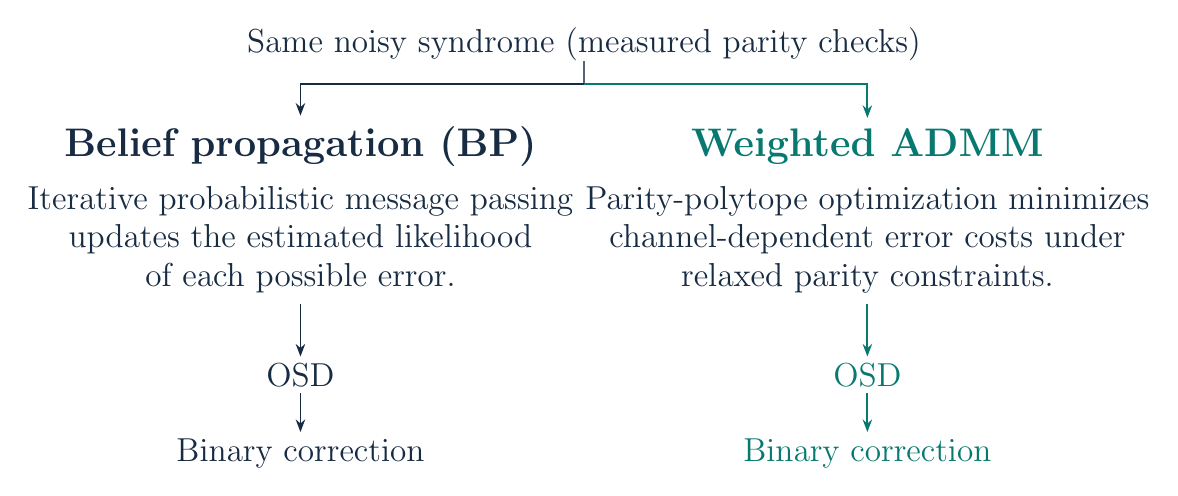
\begin{tikzpicture}[x=1mm,y=1mm]
    \node[flow text] (syndrome) at (70,52) {Same noisy syndrome (measured parity checks)};
    \coordinate (split) at (70,47);
    \draw[Muted,line width=.65pt] (syndrome.south) -- (split);
    \node[method] (bp) at (34,39) {Belief propagation (BP)};
    \node[method,text=Accent] (admm) at (106,39) {Weighted ADMM};
    \draw[flow,Ink] (split) -| ([yshift=1.4mm]bp.north);
    \draw[flow,Accent] (split) -| ([yshift=1.4mm]admm.north);

    \node[flow text,anchor=north] at (34,34)
      {Iterative probabilistic message passing\\updates the estimated likelihood\\of each possible error.};
    \node[flow text,anchor=north] at (106,34)
      {Parity-polytope optimization minimizes\\channel-dependent error costs under\\relaxed parity constraints.};
    \foreach \columnX/\branchColor in {34/Ink,106/Accent}{
      \node[flow text,text=\branchColor] (osd) at (\columnX,10) {OSD};
      \node[flow text,text=\branchColor] (binary) at (\columnX,0) {Binary correction};
      \draw[flow,\branchColor] (\columnX,19) -- ([yshift=.9mm]osd.north);
      \draw[flow,\branchColor] ([yshift=-.9mm]osd.south) -- ([yshift=.9mm]binary.north);
    }
  \end{tikzpicture}\par
  \vspace{3mm}
  \contextline{Both use the same ordered statistics decoding (OSD) step on separate error rankings.}
  \talknote[\par\medskip\footnotesize ADMM stands for alternating direction method of multipliers.
    Methods by \href{https://doi.org/10.1103/PhysRevResearch.2.043423}{Roffe et al.},
    \href{https://arxiv.org/abs/2508.04769}{Gu and Soleimanifar}, and
    \href{https://doi.org/10.1109/ISIT62367.2026.11653953}{Lyu and He}.]{2}
\end{frame}

\begin{frame}[t]{Testing the decoders on the same errors}
  \begin{columns}[c,onlytextwidth]
    \begin{column}{.34\textwidth}
      {\fontsize{35}{39}\selectfont\bfseries\color{Accent}10,000\par}
      {\fontsize{14}{17}\selectfont paired trials per setting\par}
    \end{column}
    \begin{column}{.64\textwidth}
      \centering
      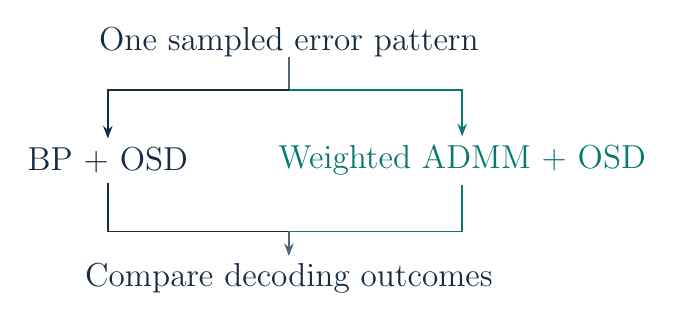
\begin{tikzpicture}[x=1mm,y=1mm]
        \node[flow text] (sample) at (44,31) {One sampled error pattern};
        \node[flow text,text=Ink] (bp) at (21,16) {BP + OSD};
        \node[flow text,text=Accent] (admm) at (66,16) {Weighted ADMM + OSD};
        \node[flow text] (compare) at (44,1) {Compare decoding outcomes};
        \coordinate (split) at (44,25);
        \coordinate (join) at (44,7);
        \draw[Muted,line width=.65pt] (sample.south) -- (split);
        \draw[flow,Ink] (split) -| ([yshift=1.2mm]bp.north);
        \draw[flow,Accent] (split) -| ([yshift=1.2mm]admm.north);
        \draw[Ink,line width=.65pt] ([yshift=-1.2mm]bp.south) |- (join);
        \draw[Accent,line width=.65pt] ([yshift=-1.2mm]admm.south) |- (join);
        \draw[flow,Muted] (join) -- ([yshift=1mm]compare.north);
      \end{tikzpicture}
    \end{column}
  \end{columns}
  \vspace{4mm}
  {\fontsize{13}{16}\selectfont\bfseries Phenomenological noise\par}
  \vspace{1.5mm}
  {\fontsize{12}{15}\selectfont
  \begin{tabular}{@{}l@{\hspace{7mm}}l@{}}
    \color{Muted}Physical data qubits & 72 or 144\\[.8mm]
    \color{Muted}Physical error rate & 0.5\%, 1\% or 2\%\\[.8mm]
    \color{Muted}Measurements & Six noisy rounds, then a perfect terminal syndrome
  \end{tabular}\par}
  \talknote[\par\medskip\footnotesize Bivariate bicycle codes by
    \href{https://doi.org/10.1038/s41586-024-07107-7}{Bravyi et al.}]{3}
\end{frame}

\begin{frame}[t]{A modest gain in one tested regime}
  \contextline{72 data qubits, 2\% phenomenological noise, six noisy rounds, greedy OSD}
  \vspace{3mm}
  \begin{tikzpicture}[
    every node/.style={inner sep=0pt,font=\fontsize{11.5}{14}\selectfont,text=Ink},
    colhead/.style={text=Muted,font=\fontsize{9.5}{12}\selectfont},
  ]
    \begin{axis}[
      at={(76mm,0)},anchor=south west,width=60mm,height=26mm,scale only axis,
      xmin=2.45,xmax=3.85,ymin=0.55,ymax=3.45,
      xtick={2.5,3,3.5},xticklabels={2.5\%,3.0\%,3.5\%},
      ytick=\empty,axis x line*=bottom,axis y line=none,
      axis line style={draw=LightRule},xtick style={draw=LightRule},
      tick label style={font=\fontsize{9.5}{12}\selectfont,text=Muted,inner sep=2pt},
      xmajorgrids=true,grid style={draw=LightRule,line width=0.4pt},
    ]
      \plotdecoder{bp}{Ink}{*}
      \plotdecoder{admm}{Muted}{square*}
      \plotdecoder{admm-w}{Accent}{diamond*}
      \coordinate (bpRow) at (axis cs:2.45,3);
      \coordinate (admmRow) at (axis cs:2.45,2);
      \coordinate (weightedRow) at (axis cs:2.45,1);
    \end{axis}
    \node[colhead,anchor=west] at (0,29mm) {Decoder};
    \node[colhead,anchor=east] at (49mm,29mm) {Block failures / 10,000};
    \node[colhead,anchor=east] at (67mm,29mm) {Rate};
    \node[colhead,anchor=west] at (76mm,29mm) {Exact 95\% confidence interval};
    \foreach \row/\decoder/\count/\rate/\ink in {
        bpRow/BP/\BPFailures/\BPRate/Ink,
        admmRow/Plain ADMM/\PlainFailures/\PlainRate/Ink,
        weightedRow/Weighted ADMM/\WeightedFailures/\WeightedRate/Accent}{
      \node[anchor=west,text=\ink] at (0,0 |- \row) {\decoder};
      \node[anchor=east,text=\ink] at (49mm,0 |- \row) {\count};
      \node[anchor=east,text=\ink] at (67mm,0 |- \row) {\rate\%};
    }
  \end{tikzpicture}\par
  \vspace{2.5mm}
  {\fontsize{14.5}{18}\selectfont
    {\bfseries\color{Accent}\the\numexpr\BPFailures-\WeightedFailures\relax{} fewer failures} than BP,
    a \RelativeReduction\% relative reduction.\par}
  \vspace{1.5mm}
  \contextline{Only 1 of 24 primary comparisons was significant after Holm adjustment ($p=\AdjustedP$).}
  \talknote[\par\medskip\footnotesize Points show observed rates. Bars show marginal
    exact 95\% binomial intervals. The adjusted $p$-value uses a paired exact McNemar test.
    Data from qudec campaign 21501046.]{4}
\end{frame}

\begin{frame}[t]{Circuit-level noise and next steps}
  \relax
  {\fontsize{14}{17}\selectfont BP + OSD had fewer failures in all four preliminary circuit tests.\par}
  \vspace{1mm}
  \contextline{These runs used untuned ADMM. The effect of circuit-specific tuning is still open.}
  \vspace{4mm}

  \begin{columns}[T,onlytextwidth]
    \begin{column}{0.56\textwidth}
      {\fontsize{12}{15}\selectfont\bfseries Block failures per 300 trials\par}
      \vspace{1mm}
      \begin{tikzpicture}
        \begin{axis}[
          width=51mm,height=30mm,scale only axis,
          xmin=0,xmax=57,ymin=0.6,ymax=4.4,y dir=reverse,
          xtick={0,10,20,30,40,50},ytick={1,2,3,4},
          yticklabels={{Z memory, 0.1\%},{Z memory, 0.2\%},{X memory, 0.1\%},{X memory, 0.2\%}},
          xticklabels={0,10,20,30,40,50},
          axis x line*=bottom,axis y line*=left,y axis line style={draw=none},
          axis line style={draw=LightRule},ytick style={draw=none},xtick style={draw=LightRule},
          tick label style={font=\fontsize{9}{11}\selectfont,text=Ink},
          xmajorgrids=true,grid style={draw=LightRule,line width=0.4pt},
          nodes near coords={\pgfmathprintnumber[assume math mode=true]{\pgfplotspointmeta}},
          every node near coord/.append style={anchor=west,xshift=.6pt,font=\fontsize{9.5}{11}\selectfont},
          legend style={at={(0.5,-0.24)},anchor=north,draw=none,fill=none,
            font=\fontsize{9}{11}\selectfont,/tikz/every even column/.append style={column sep=2mm}},
          legend columns=2,
        ]
          \addplot[only marks,mark=*,mark size=2.5pt,Ink,point meta=x]
            table[x=failures,y=x,col sep=comma] {build/circuit_bp.csv};
          \addlegendentry{BP + OSD}
          \addplot[only marks,mark=diamond*,mark size=3.4pt,Accent,point meta=x]
            table[x=failures,y=x,col sep=comma] {build/circuit_admm.csv};
          \addlegendentry{ADMM + OSD}
        \end{axis}
      \end{tikzpicture}
    \end{column}
    \begin{column}{0.40\textwidth}
      {\fontsize{12}{15}\selectfont\bfseries\color{Accent}Next steps\par}
      \vspace{2mm}
      {\fontsize{11}{14}\selectfont
        Replicate the phenomenological result on independent samples.\par\vspace{2mm}
        Tune ADMM for circuit-level noise.\par\vspace{2mm}
        Run more trials to narrow the confidence intervals.\par}
    \end{column}
  \end{columns}
  \talknote[\par\medskip\footnotesize Circuit data from qudec campaign 21501046.
    The 72-qubit circuit used three rounds. X and Z denote memory bases, with physical
    error rates of 0.1\% and 0.2\%. The held-out runs used a different OSD setting.]{5}
\end{frame}

\end{document}
